\chapter{Design of Laha}

Laha, which means, to spread or distribute in Hawaiian, is an abstract framework for distributed sensor networks that provides a means for big data management as well as augmenting a DSN with the ability to adaptively optimize its bandwidth, detection, classification, and sensor device power requirements.

The Laha framework is made up of five layers that can be viewed conceptually as a pyramid (see \ref{laha-figure}). Data entering the Laha framework is located at the bottom the bottom of the pyramid. As data moves upward through the layers, noise is discarded, less interesting events are discarded or aggregated into upper layers, events are given more meaning and context, and associations and predictions are made. 

\begin{figure}
\caption{Laha Conceptual Model}
\centering
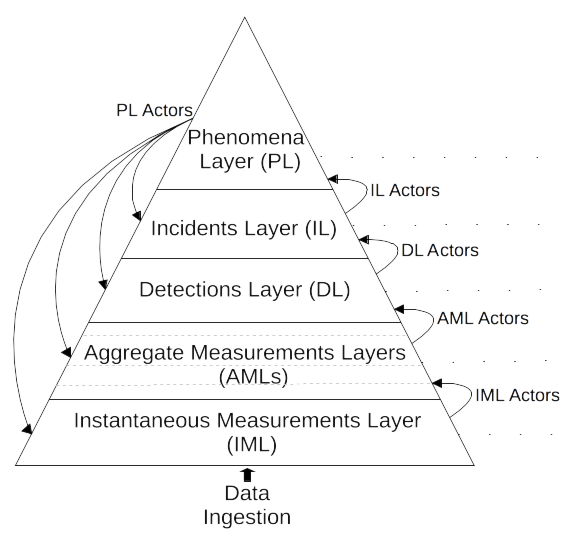
\includegraphics{figures/laha.png}	
\label{laha-figure}
\end{figure}

\section{Big Data Management in Laha} \label{big-data-management}
The Laha framework acts as an adaptive sieve for filtering noise and uninteresting data collected from a DSN. In this way, each layer only passes what it considers interesting to the layer above it. All data at a particular layer is garbage collected at specific intervals relating to its important to the DSN.

Each layer only keeps data for a specified amount of time before it is garbage collected. As data moves up the pyramid, it is generally considered more useful and therefore has a longer Time to Live (TTL), the amount of the time the data lives before it is garbage collected.  When a higher layer detects ``something interesting", the data contained in the time window of ``something interesting" is copied into the layers above it and will still persist even though the original data is garbage collected. In this way, we preserve data from all layers if they are associated with interesting data. 

A summary of how data management in Laha is provided in table \ref{data-managament-table}. Note that the TTL is configurable for each implementing network and the table provides default values.

\begin{table}
	\caption{Summary of data management in Laha}
	\begin{tabular}{|c|c|c|}
		\hline 
		Layer & Description & Time-to-Live (TTL) \\ 
		\hline 
		Phenomena Layer (PL) & Contextual \& predictive analytics &  \\ 
		\hline 
		Incidents Layer (IL) & Classified signals &  1 year \\ 
		\hline 
		Detections Layer (DL) & Triggered windowed raw data & 1 week  \\ 
		\hline 
		Aggregate Measurements Layer (AML) & Statistical aggregates of raw data  & 1 day  \\ 
		\hline 
		Instantaneous Measurements Layer (IML) & Raw sensor data  & 1 hour \\ 
		\hline 
	\end{tabular} 
    \label{data-managament-table}
\end{table}

\subsection{Instantaneous Measurements Layer}
The Instantaneous Measurements Layer (IML) receives raw, sampled data from the DSN. The amount of data received is determined by the sample rate of each device multiplied by the number of fields per sample. Most of the time samples, from devices in the network are mainly sampling noise. A large percentage of the data in this layer is destined for garbage collection and data is assigned a Time to Live (TTL) of one hour. 


\subsection{Aggregate Measurements Layer}
The Aggregate Measurements Layer (AML) is responsible for rolling up IMs from the IML. In general, this layer only works with feature extracted data, rather than working with the raw samples. Each measurement in the AML provides summary statistics over a configurable time window. For example, these can include min, max, mean, median, mode, and variance statistics. 

It's possible to breakup the AML into several sub layers, each with different window sizes. For example, we might roll IMs into one minute AMs, then roll one minute AMs into hour AMs, then days, and so on. Each sublayer within the AML can have its own configurable TTL, ensuring long term summary statistics stick around for as long as needed. This provides us a high level view of the network and can provide insights into long term trends which wouldn't be visible (or available) in the IM data stream.

Similar to IMs, AMs can be saved and copied to the layers above it when interesting data is observed. This ability allows for AMs during these time periods to be stored and saved from the garbage collection process.

At this point in the hierarchy, we are still not providing any context to the data that we are receiving. Context is provided by layers above the AML.

\subsection{Detections Layer}
The Detections Layer (DL) is the first layer that provides some context to the data that the sink is receiving. This layer is responsible watching the feature extracted data streams, and requesting IMs from the IM layer. In general, the detection layer is meant to be trigger happy\footnote{Pun intended.} and be overly aggressive when determining if a feature extracted data stream looks interesting. 

When a data stream looks interesting, the DL marks a timestamp $N$ seconds before the interesting features and $M$ seconds after the interesting features, where both $N$ and $M$ are configurable within the framework. The goal is to use a time window that catches signals of interest within it. Since these data ranges will be further processed and refined higher in the hierarchy, there is no issue with collecting larges amounts of data in this layer. 

The actual methods of detection is dependent on the characteristics of every individual sensor network. This framework assumes that the detection algorithms are provided by the implementing frameworks.

Similar to other layers, the DL layer will have its IMs and AMs copied into layers above it when upper layers observe something interesting in the DL. The detections layer is set to have a TTL of a week.

\subsection{Incidents Layer}
Incidents represent classified signals. Incidents are individual classifications for signals of interest and are created by analyzing waveforms from Events. Waveforms from Events may contain multiple incidents. Individual signals may be classified as multiple incidents (for example a transient being classified as both a transient and frequency incidents). 

Incidents are further analyzed to produce phenomena. 

Incidents are expired after one year of storage. 


\subsection{Phenomena Layer}
Phenomena are defined as a grouping of incidents that provide one or more of annotations, locality, periodicity, predictiveness, similarity, and future phenomena. 

Not only do Phenomena provide interesting insight and analytics into the underlying data, but they also provide a means for adaptively tuning the underlying collection, triggering, detection, and analysis of a distributed sensor network.

Phenomena are summarized in table \ref{phenomena-summary-table} and discussed in great detail in section \ref{phenomena}.

\section{Phenomena: Providing Adaptive Optimizations in Laha} \label{phenomena}

\begin{table}
	\centering
	\caption{Summary of Laha Phenomena}
	\begin{tabular}{|c|c|}
		\hline
		Phenomena & Description \\
		\hline
		Annotations & Provide context about an Incident or set of incidents \\
		\hline
		Locality & Provides context on how incidents are related in time and space \\
		\hline
		Periodicity & Designation for incidents that exhibit repetitive or periodic behavior \\ 
		\hline
		Similarity & Subset of incidents found using grouping and community detection algorithms \\
		\hline
		Predictive & Subset of incidents characterized by predictive or forecasting models\\
		\hline
		Future & Incidents scheduled to occur in the future\\
		\hline
	\end{tabular}
	\label{phenomena-summary-table}
\end{table}

\subsection{Annotations Phenomena} \label{annotations-phenomena}
Annotations provide context about an Incident or a set of Incidents. Annotations are generally user provided or sourced from other data sources to provide supporting context to Incidents. For example, Annotations might include “Cloud Cover”, “Hurricane Hector”, “Dryer Turns On”, etc.

In some sense, annotations allow us to label our data sets beyond a simple classification and start looking at causal classifications. Once enough annotations have been assigned to classified incidents, Laha can used Annotations to attempt to label unknown incidents with similar characteristics.

Annotations can be used to tune Laha's detection and classification algorithms by allowing Laha to filter on incidents with known causes.

\subsection{Locality Phenomena} \label{locality-phenomena}
Locality provides context on how incidents are related to each other in both space in time. Laha is able to determine if classified incidents are local to a single sensor, to a group of co-located sensors, or global across an entire network. Sensors can be co-located in both the physical sense and also co-located within a sensing field. For example, sensors in a power quality network may be separated by large distance geographically, but co-located through the electrical grid and the grid's topology. 

Over time, Locality Phenomena is used to build a model of sensors in relation to each other and to provide a statistical likelihood that co-located sensors will observe the same signal. Locality phenomena can be used to drive network triggering, detection, and classification thresholds within a distributed sensor network by using this probabilistic model for determining the likelihood that a sensor or sensors will observe a signal of interest.

\subsection{Periodicity Phenomena} \label{periodicity-phenomena}
Periodic phenomena consists of incidents that exhibit repetitive behavior, that is, the same types of incidents appearing in cycles from single or multiple devices. Periodicity allows for the easy creation of Predictive phenomena.

Periodic phenomena can come from a single incident or from multiple incidents. Periodic phenomena allow us to either tune our network to find periodic incidents or tune the  network to ignore periodic incidents depending on if the incidents are of interest. Periodic phenomena are especially useful in conjunction with Annotation phenomena as we can assign causality to the periodic signal. 

\subsection{Similarity Phenomena}
Similarity phenomena utilize grouping and community detection algorithms to group incidents together by their features. Common features used for grouping include time, location, incident type, or incident features.

% TODO describe common community detection algorithms 

\subsection{Predictive Phenomena}
Predictive phenomena consists of incidents that are characterized by a predictive or forecasting models. Predictiveness is a behavior that can be inferred from all other phenomena types. 

Predictiveness is the main driver behind optimizing the control of a distributed sensor network. If we can predict the types of signals that will arrive at sensors, then we can tune those sensors and the sink to either filter the signals (if the user is not interested in signals) or tune the sensors and the sink to be extra sensitive to those signals, possible detecting them even if they previously would not have been detected.

\subsection{Future Phenomena}
Predictive phenomena can be used to create future phenomena. Future phenomena are a statistical model of the likelihood of seeing an incident or incidents at future points in time. Knowing that a signal may occur with some probability allows agents affected by those signals time to prepare for the signals.

\section{Laha Actors: Acting on the Laha Data Model}
Laha Actors act on the Laha hierarchy and provide one of two functions. Actors can move data from one level of the hierarchy upwards through the hierarchy when interesting data is requested by an upper level. Actors can also apply adaptive optimizations downwards through the hierarchy. The Laha framework can support multiple actors at each level. For example, the Incidents Layer in our reference power quality network contains actors for each of the following functions: IEEE classified voltage events, frequency variations, power outages, excessive THD, and many others. The Incident Layer Actors move data from these incidents upwards to the Phenomena Layer.  

Table \ref{laha-actors-tables} summarizes the actors that exist within the Laha framework and their purposes. 

\begin{table}
	\centering
	\caption{Summary of Laha Actors}
	\begin{tabular}{|c|c|}
		\hline
		Actor & Purpose \\
		\hline
		IML Actors & Perform feature extraction and move aggregate data to AML \\
		\hline
		AML Actors & Perform triggering on data from IML, copy data to DL if interesting \\
		\hline
		DL Actors & Perform high fidelity feature extraction on possible detections \\
		\hline
		IL Actors & Perform classification and contextualization on possible detections \\
		\hline
		PL Actors & Generate predictive analytics and optimize the lower levels of the hierarchy \\
		\hline
	\end{tabular}
	\label{laha-actors-tables}
\end{table}

\subsection{Actor Constraints}
Actors at each level in the hierarchy are governed by a set of constraints. These constraints include the set of possible inputs, $A_i$, the set of possible outputs, $A_o$, the set of Actors it can receive data from, $A_{ai}$, the set of Actors it can transmit data to, $A_{ao}$, and a set of performance metrics that each actor must maintain, $A_p$. The constraints assigned to each Actor are determined by the hierarchy level in which the Actor resides.  

Actors are responsible for reporting constraint violations and in this way, Actors are the primary provider of health, performance, and status metrics about the Laha framework.

The constraints for each level of Laha hierarchy is summarized in table \ref{actor-constraint-table}.

\begin{table}
	\centering
	\caption{Summary of Laha Actor Constraints at Each Level}
	\begin{tabular}{|c|c|c|c|c|c|}
		\hline
		Level & $A_i$ & $Ao$ & $A_{ai}$ & $A_{ao}$ & $A_p$ \\
		\hline
		IML & Raw samples & Aggregate trends & n/a & AML & Data ranges available \\
		\hline
		AML & Aggregate trends & Detections & IML & DL & Data ranges available \\
		\hline
		DL & Windowed waveforms & Hi-fi extracted features & AML & IL & Data \& features available \\
		\hline
		IL & Hi-fi extracted features & Contextualized incidents & DL & PL & Incident types available \\
		\hline
		PL & Contextualized incidents & Optimizations & IL & All levels & Optimizations available \\
		\hline
	\end{tabular}
	\label{actor-constraint-table}
\end{table}